\documentclass[polish,a4paper]{article}
\usepackage{amsmath}
\usepackage{amssymb, amsfonts, amsthm, amsmath, bm}
\usepackage[T1]{fontenc}
\usepackage[utf8]{inputenc}
\usepackage{babel}
\usepackage{pslatex}
\usepackage{pgfplots}
\usepackage{hhline}
\usepackage[american]{circuitikz} 
\usepackage{anysize}
\usepackage{graphicx}
\DeclareGraphicsExtensions{.jpg}
\marginsize{2.5cm}{2.5cm}{3cm}{3cm}
\bibliographystyle{IEEEtran}


%makro do indeksów w tabeli
\newcommand{\PRzFieldDsc}[1]{\sffamily\bfseries\scriptsize #1}

%makro do informacji w tabeli
\newcommand{\PRzFieldCnt}[1]{\itshape #1}

%potężne makro tworzące tabelę z informacjami o teamie
\newcommand{\PRzHeading}[8]{
%% #1 - nazwa laboratorium
%% #2 - kierunek 
%% #3 - specjalność 
%% #4 - rok studiów 
%% #5 - symbol grupy lab.
%% #6 - temat 
%% #7 - numer lab.
%% #8 - skład grupy ćwiczeniowej

\begin{center}
\begin{tabular}{ p{0.32\textwidth} p{0.15\textwidth} p{0.15\textwidth} p{0.12\textwidth} p{0.12\textwidth} }

  &   &   &   &   \\
\hline
\multicolumn{5}{|c|}{}\\[-1ex]
\multicolumn{5}{|c|}{{\LARGE #1}}\\
\multicolumn{5}{|c|}{}\\[-1ex]

\hline
\multicolumn{1}{|l|}{\PRzFieldDsc{Kierunek}}	& \multicolumn{1}{|l|}{\PRzFieldDsc{Specjalność}}	& \multicolumn{1}{|l|}{\PRzFieldDsc{Rok studiów}}	& \multicolumn{2}{|l|}{\PRzFieldDsc{Symbol grupy lab.}} \\
\multicolumn{1}{|c|}{\PRzFieldCnt{#2}}		& \multicolumn{1}{|c|}{\PRzFieldCnt{#3}}		& \multicolumn{1}{|c|}{\PRzFieldCnt{#4}}		& \multicolumn{2}{|c|}{\PRzFieldCnt{#5}} \\

\hline
\multicolumn{4}{|l|}{\PRzFieldDsc{Temat Laboratorium}}		& \multicolumn{1}{|l|}{\PRzFieldDsc{Numer lab.}} \\
\multicolumn{4}{|c|}{\PRzFieldCnt{#6}}				& \multicolumn{1}{|c|}{\PRzFieldCnt{#7}} \\

\hline
\multicolumn{5}{|l|}{\PRzFieldDsc{Skład grupy ćwiczeniowej oraz numery indeksów}}\\
\multicolumn{5}{|c|}{\PRzFieldCnt{#8}}\\

\hline
\multicolumn{3}{|l|}{\PRzFieldDsc{Uwagi}}	& \multicolumn{2}{|l|}{\PRzFieldDsc{Ocena}} \\
\multicolumn{3}{|c|}{\PRzFieldCnt{\ }}		& \multicolumn{2}{|c|}{\PRzFieldCnt{\ }} \\

\hline
\end{tabular}
\end{center}
}
%koniec potężnego makro do tabeli

\begin{document}

%stworzenie tabeli - miejsce na zmienianie danych w tabeli
%indeksy do uzupełnienia
\PRzHeading{Laboratorium Podstaw Elektroniki}{Informatyka}{--}{I}{I1}{Diody}{4}{Ewa Fengler(132219), Sebastian Maciejewski(132275), Jan Techner(132332)}{}

%ZADANIA

\section*{Cel}
Celem przeprowadzanych doświadczeń jest zapoznanie się z układami diodowymi dzięki badaniu charakterystyki diody złączowej, konstrukcji prostownika jednopołówkowego oraz budowaniu obwodów zawierających diody świecące.

\section{Zadanie 1.2}


\subsection*{2.}
Rzeczywiste wartości rezystancji wykorzystanych elementów:

\begin{center}
\begin{tabular}{|c||c|c|c|c|}
\hline
\textbf{Element} & \textbf{Wartość zadana} & \textbf{Oznaczenie} & \textbf{Odczyt} & \textbf{Wartość zmierzona}\\
\hhline{|=#=|=|=|=|}
\textbf{R1} & 1k$\Omega$ & brązowy, czarny, czerwony, złoty & $1k\Omega\pm5\%$ & $984,3\Omega$\\
\hline
\textbf{R2} & 3M$\Omega$ & pomarańczowy, czarny, zielony, złoty & $3M\Omega\pm5\%$ & $3,009M\Omega$\\
\hline
\end{tabular}
\end{center}


\subsection*{3.}

\begin{figure}[!h]
\centering
\begin{circuitikz}[scale=0.9, font = \scriptsize, european voltages]
\draw (0,-1) to [american current source, o-o, v>=$U_z$] (0,1) to [stroke diode, l=$D1$, v<=$U_d$, o-*] (3,1) to [R,*-*, v<=$U_{R_1}$] (3,-1) -- (0,-1)
	  (3,1) -- (4.5,1) to [voltmeter] (4.5,-1) -- (3,-1);
	  
	  
\draw (3.5, 0.2) node {$R_1$}
	  (3.5, -0.2) node {1k$\Omega$}
	  ;

\end{circuitikz}
\caption{Układ do badania charakterystyki statycznej diody PN - kierunek przewodzenia}
\label{fig:badobw}
\end{figure}

\newpage
\subsection*{4.}
\begin{flushleft}
Pomiary spadków napięć $U_{R1}$ na rezystorze zmierzone dla wartości napięcia źródła $U_{z}$ w zakresie $0 - 5V$ oraz obliczone wartości napięć na zaciskach diody $U_{d}$ i wartości prądów diody $I_{d}$ wyrażone jako odpowiednio:
\end{flushleft}

$$
U_{d} = U_{z} - U_{R_1}
$$

$$
I_{d} = \frac{U_{R_1}}{R1}
$$

\begin{flushleft}
gdzie $R$ jest rzeczywistą (zmierzoną) wartością rezystancji opornika $R_1$ wykorzystanego do konstrukcji układu.\\
Wyniki zaokrąglono do dwóch miejsc po przecinku.
\end{flushleft}

\begin{center}
\begin{tabular}{|c|c||c|c|}
\hline
\boldsymbol{$U_z$} [V] & \boldsymbol{$U_{R_1}$} [V] & \boldsymbol{$U_d$} [V]& \boldsymbol{$I_d$} [mA]\\
\hhline{|=|=#=|=|}
0 & 0 & 0 & 0\\ \hline
0,2 & 0,01 & 0,19 & 0,01\\ \hline
0,4 & 0,11 & 0,29 & 0,11\\ \hline
0,6 & 0,27 & 0,33 & 0,27\\ \hline
0,8 & 0,42 & 0,38 & 0,43\\ \hline
1 & 0,58 & 0,42 & 0,59\\ \hline
1,5 & 1,06 & 0,44 & 1,08\\ \hline
2 & 1,57 & 0,43 & 1,60\\ \hline
2,5 & 2,09 & 0,41 & 2,12\\ \hline
3 & 2,61 & 0,39 & 2,65\\ \hline
3,5 & 3,03 & 0,47 & 3,08\\ \hline
4 & 3,51 & 0,49 & 3,57\\ \hline
4,5 & 4,03 & 0,47 & 4,09\\ \hline
5 & 4,55 & 0,45 & 4,26\\ \hline

\end{tabular}
\end{center}

\subsection*{5.}
\begin{figure}[!h]
\centering
\begin{circuitikz}[scale=1.1, font = \scriptsize, european voltages]
\draw (0,-1) to [american current source, o-o, v>=$U_z$] (0,1)
(3,1) to [stroke diode, l_=$D1$, v^>=$U_d$, o-*] (0,1)
(3,1) to [R,*-*, v<=$U_{R_2}$] (3,-1) -- (0,-1)
	  (3,1) -- (4.5,1) to [voltmeter] (4.5,-1) -- (3,-1);
	  
	  
\draw (3.5, 0.2) node {$R_2$}
	  (3.5, -0.2) node {3M$\Omega$}
	  ;

\end{circuitikz}
\caption{Układ do badania charakterystyki statycznej diody PN - kierunek zaporowy}
\label{fig:badobw}
\end{figure}

\subsection*{6.}
\begin{flushleft}
Podobnie jak w podpunkcie 4., w tabeli przedstawiono pomiary spadków napięć $U_{R}$ na rezystorze $R_2$ (dla wyznaczonej doświadczalnie wartości jego rezystancji) zmierzone dla wartości napięcia źródła $U_{z}$ w zakresie $0 - 20V$ oraz obliczone wartości napięć na zaciskach diody $U_{d}$ i wartości prądów diody $I_{d}$ wyrażone wzorami przedstawionymi w podpunkcie 4.\\
Wyniki zaokrąglono do dwóch miejsc po przecinku, za wyjątkiem $U_{d}$, którego wartości zaokrąglono do trzech miejsc po przecinku. 

\end{flushleft}

\begin{center}
\begin{tabular}{|c|c||c|c|}
\hline
\boldsymbol{$U_z$} [V] & \boldsymbol{$U_R$} [mV] & \boldsymbol{$U_d$} [V]& \boldsymbol{$I_d$} [$\mu A$]\\
\hhline{|=|=#=|=|}
0 & 0 & 0 & 0\\ \hline
5 & 3,35 & 4,999 & 1,11\\ \hline
10 & 3,94 & 9,996 & 1,31\\ \hline
15 & 4,52 & 14,995 & 1,50\\ \hline
20 & 4,75 & 19,995 & 1,58\\ \hline
\end{tabular}
\end{center}



\subsection*{9.}

\begin{figure}[!h]
\centering
\begin{tikzpicture}[scale=1]
\begin{axis}[
xlabel={Napięcie na źródle [V]},
ylabel={Prąd diody [mA]},
xmin=0,xmax=22,
ymin=0,ymax=5,
legend pos=north east,
ymajorgrids=true,grid style=dashed
]

%Vrms - napięcie na źródle
\addplot[smooth, tension={0.8}, red, mark=*, mark size = {1pt}]
coordinates {
(0,0)
(0.2,0.01)
(0.4,0.11)
(0.6,0.27)
(0.8,0.43)
(1,0.59)
(1.5,1.08)
(2,1.6)
(2.5,2.12)
(3, 2.65)
(3.5,3.08)
(4,3.57)
(4.5,4.09)
(5,4.26)
};

%napięcie na rezystorze
\addplot[smooth, tension={0.8}, cyan, mark=*, mark size = {1pt}]
coordinates {
(0,0)
(5,1.11)
(10,1.31)
(15,1.5)
(20,1.58)
};
\legend{kierunek przewodzenia,kierunek zaporowy}
\end{axis}
\end{tikzpicture}
\caption{Przebieg charakterystyki $I_d = f(U_z)$ dla diody spolaryzowanej w kierunku zaporowym i przewodzenia}
\label{fig:wyk}
\end{figure}

\newpage
\section{Zadanie 1.3}


\subsection*{1.}

\begin{figure}[!h]
\centering
\begin{circuitikz}[scale=1.1, font = \scriptsize]
\draw (0,1) to [sinusoidal voltage source, l^=sinus, o-o] (0,-1)
	  (0,1) to [stroke diode, l_=$D2$, o-*] (2,1) to [R, l_=$R$, a^=10k$\Omega$, *-*] (2, -1) -- (0,-1)
	  (2,1) -- (3.5,1) to [short, -o] (3.5, 0.3) -- (3.8, 0.3) 
	  (2,-1) -- (3.5,-1) to [short, -o] (3.5, -0.3) -- (3.8, -0.3)
	  (0,1) -- (0, 3) to [short, -o] (1, 3)
	  (1,2.4) to [short, o-] (0.5, 2.4) 
	  (1,2.4) -- (1.3, 2.4)
	  (1,3) -- (1.3, 3) 
	  ; 
\draw

	  (2,-1.5) node {GND}
	  (0.5,1.9) node {GND}
   
      (-1, 0) node {f = 50Hz} 
      (2,-1) node [rground] {}
      (0.5,2.4) node [rground] {}
      (4, 0) node[rotate=90] {\small\textbf{kanał B}}
      (1.5, 2.7) node[rotate=90] {\small\textbf{kanał A}}
	  ;
\end{circuitikz}
\caption{Układ pomiarowy dla badania własności prostownika jednopołówkowego}
\label{fig:badobw}
\end{figure}

\newpage

\subsection*{2.} 

Oscylogram kształtu przebiegu na wejściu i wyjściu prostownika.\\

\includegraphics[width=\textwidth]{50hz}



\subsection*{3.} Różnica amplitud napięcia między przebiegiem wejściowym oraz wyjściowym:

\begin{center}
\begin{tabular}{|l|l|}
\hline
$V_{RMS1}$ & 1,64V \\
\hline
$V_{RMS2}$ & 0,7V \\ 
\hline
różnica & 0,96V \\
\hline
\end{tabular}
\end{center}

\begin{flushleft}
Różnica między napięciami wynika z faktu, iż badany układ, jako prostownik jednopołówkowy, dokonuje częściowego wyprostowania płynącego prądu - zmienia go z prądu przemiennego na prąd tętniący, czyli prąd przemienny, z którego "usuwamy" ujemne wartości napięcia.
\end{flushleft}

\newpage

\subsection*{4.}


\begin{figure}[!h]
\centering
\begin{circuitikz}[scale=1.1, font = \scriptsize]
\draw (0,1) to [sinusoidal voltage source, l_=sinus, o-o] (0,-1)
	  (0,1) to [stroke diode, l_=$D$, o-*] (2,1) to [R, l_=$R$, *-*] (2, -1) -- (0,-1)
	  (2,1) -- (7.5,1) to [short, -o] (7.5, 0.3) -- (7.8, 0.3) 
	  (2,-1) -- (7.5,-1) to [short, -o] (7.5, -0.3) -- (7.8, -0.3)
	  (0,1) -- (0, 3) to [short, -o] (1, 3)
	  (1,2.4) to [short, o-] (0.5, 2.4) 
	  (1,2.4) -- (1.3, 2.4)
	  (1,3) -- (1.3, 3) 
	  
	  (3.5,1) to [ecapacitor, l=CF] (3.5,-1)
	  (5,1) to [esource] (5,-1)
	  (6.3,1) to [esource] (6.3,-1)
	  ; 
\draw

	  (2,-1.5) node {GND}
	  (0.5,1.9) node {GND}
   	  (5,0) node {$V_{AC}$}
   	  (6.3,0) node {$V_{DC}$}
      (2,-1) node [rground] {}
      (0.5,2.4) node [rground] {}
      (8, 0) node[rotate=90] {\small\textbf{kanał B}}
      (1.5, 2.7) node[rotate=90] {\small\textbf{kanał A}}
	  ;
\end{circuitikz}
\caption{Układ prostownika jednopołówkowego z filtracją}
\label{fig:badobw}
\end{figure}

\subsection*{6.}

Napięcia stałe oraz zmienne na rezystancji $R$, wraz z wartościami międzyszczytowymi napięcia tętnień na rezystancji R, dla danych kombinacji elementów.


\begin{center}
\begin{tabular}{|c|c||c|c|c|}
\hline
\boldsymbol{$R [\Omega]$} & \boldsymbol{$C_f [\mu F]$} & \boldsymbol{$U_{R(DC)} [V]$} & \boldsymbol{$U_{R(AC)} [V]$} & \boldsymbol{$U_{R(pp)} [V]$} \\
\hhline{|=|=#=|=|=|}
2200 & 2,2 & 3,897 & 0,436 & 1,5 \\
\hline
220	& 2,2 & 1,550 & 1,167 & 3,52 \\
\hline
220 & 20 & 2,199 & 0,236 & 0,8 \\
\hline
2200 & 20 & 3,975 & 0,050 & 0,18 \\
\hline
\end{tabular}
\end{center}

%Niby jednostki sa u gory, ale jak uznacie, ze czytelniej z jednostkami, to mozecie dopisac


\subsection*{8.} [Interpretacja] 
% Jakie zależności można dostrzec pomiędzy wielkością napięcia międzyszczytowego tętnień, wartością pojemności filtrującej Cf oraz wartością rezystancji obciążenia R?

\subsection*{9.} [Interpretacja, Teoria(?)]
% Jaka jest interpretacja pomiarów napięcia stałego (DC) oraz zmiennego (AC) w układach prostownikowych?
\newpage

\section{Zadanie 1.4}


\subsection*{1.}
\begin{figure}[!h]
\centering
\begin{circuitikz}[scale=1.1, font = \scriptsize, european voltages]
\draw (0,-1) to [american current source, o-o] (0,1)
(0,1) to [stroke led, l_=$LED1$] (2,1) to [stroke led, l_=$LED2$] (4,1) to [R, l_=$R_1$, a^=1k$\Omega$] (4,-1) to (0,-1)
	  (0.2,1) -- (0.2,2.5) to [voltmeter] (1.8, 2.5) -- (1.8, 1) 
	  (2.2,1) -- (2.2, 2.5) to [voltmeter] (3.8,2.5) -- (3.8, 1)
;
	  
	  
	  
\draw (1,0.2) node {green}
	  (3,0.2) node {red}
	  (2,-1) node [rground] {}
	  (2,-1.5) node {GND}
	  ;

\end{circuitikz}
\caption{Schemat układu pomiarowego do badania diod świecących}
\label{fig:badobw}
\end{figure}

\subsection*{2.}
Wpływ wartości napięcia zasilania na świecenie diod.\\
Na zdjęciach przedstawiono świecenie diod dla napięć $5V$, $10V$ oraz $15V$.\\
\\
\textbf{1. $5V$}\\
\\
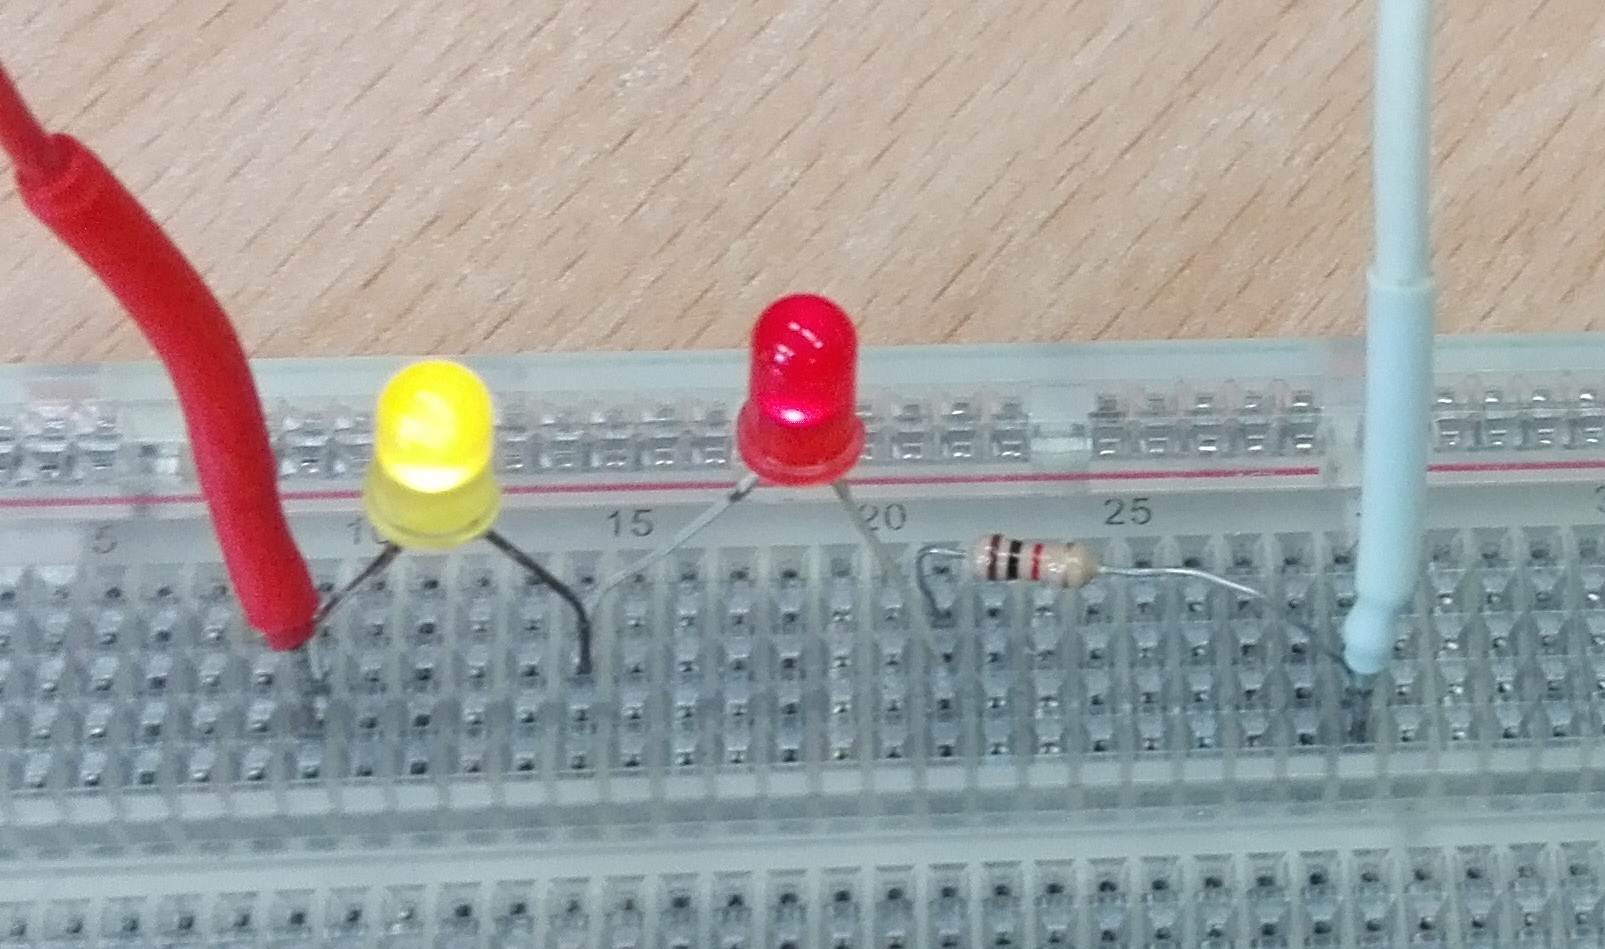
\includegraphics[width=\textwidth]{5v}
\\
\newpage
\textbf{2. $10V$}\\
\\
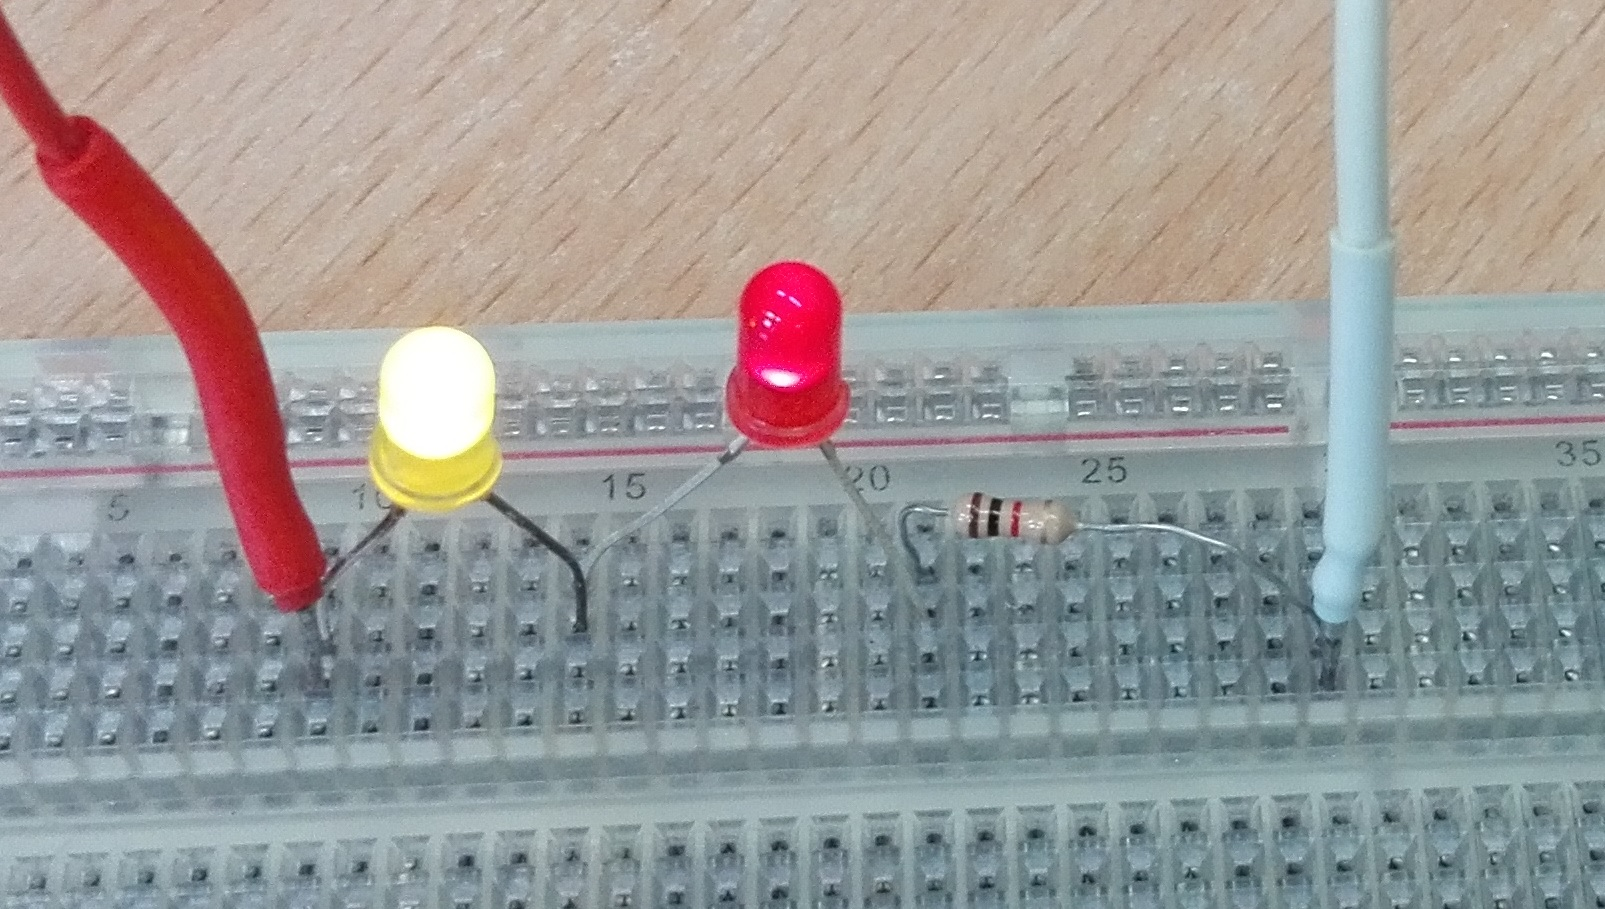
\includegraphics[width=\textwidth]{10v}
\\
\\
\textbf{3. $15V$}\\
\\
\includegraphics[width=\textwidth]{15V}
\\

%Uruchom układ pomiarow. Zaobserwuj wpływ wartości napięcia zasilania na intensynowść świecenia diod.


\subsection*{3.} Spadki napięć na obu świecących diodach:
%Przy pomocy woltomierza napięcia stałego zmierz wartości spadków napięć na obu świecacych diodach. Pomiaru dokonaj z dokładnością przy najmniej 1mV .
\newline

Spadek na diodzie żółtej: 1,967V
\newline

Spadek na diodzie czerwonej: 2,036V
\newline


\subsection*{4.} [Wyjaśnienie]
%Wyjaśnij zależność między zmierzonymi spadkami napięcia a kolorem świecenia diody.

\section{Zadanie 1.5}
Cyfrą, którą mieliśmy uzyskać na wyświetlaczu była cyfra 6, poniżej przedstawiono zdjęcie i schemat połączeń niezbędnych do otrzymania takiego obrazu na wyświetlaczu.\\
\\
\textbf{Zdjęcie wyświetlacza}\\
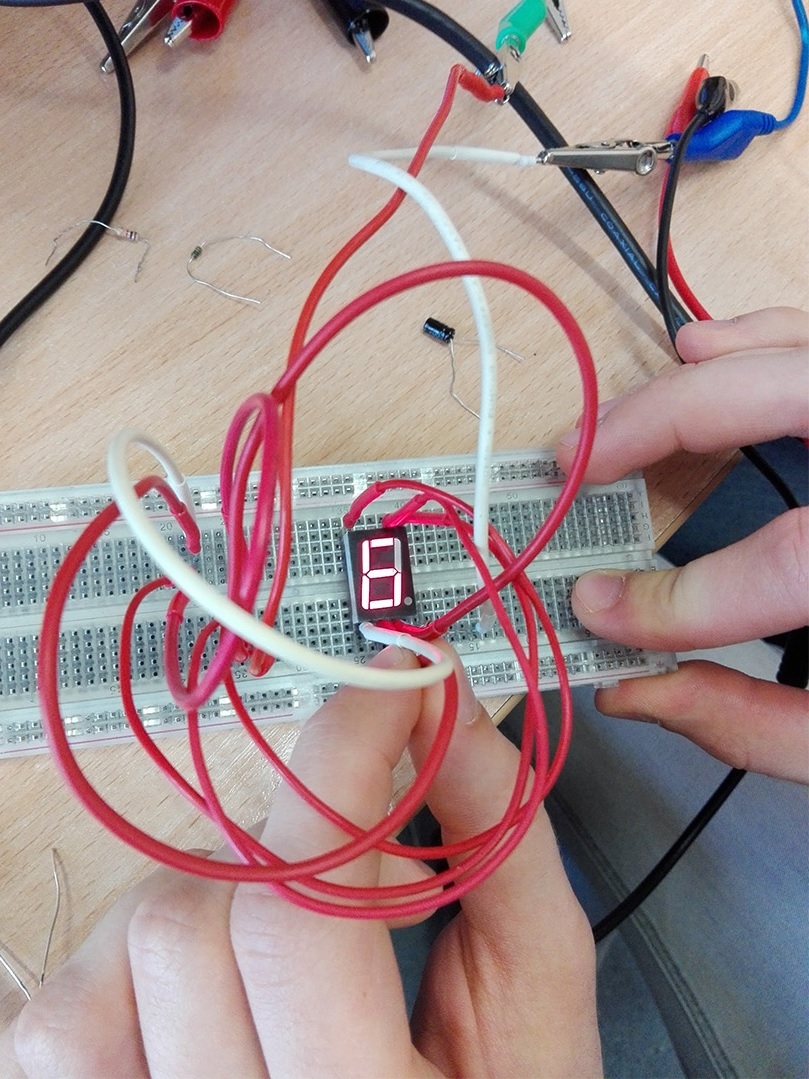
\includegraphics[width=\textwidth]{cyfra2}




[Schemat połączeń D:]


\bibliography{IEEEabrv,refs}

\begin{thebibliography}{9}

\bibitem{rlc}
  W trakcie przeprowadzania doświadczeń i pisania sprawozdania zespół korzystał głównie z materiałów ze strony http://etacar.put.poznan.pl/mariusz.naumowicz/materialy.html oraz z wiedzy własnej.

\end{thebibliography}

\end{document}7